\graphicspath{{chapters/method/figures/}}

\subsection{forumulation}
\begin{frame}\frametitle{Optimization}
\framesubtitle{For image segmentation}

\begin{equation*}
\hat{\omega} = \arg \min_{\substack{\omega}} \,U(\omega)
\end{equation*} 

\begin{block}{Considerations}
  \begin{itemize}
    \item Search Space $\mathcal{W}$
    \item Cost Function $U(\cdot)$
      \item Minimization Strategy
  \end{itemize}
\end{block}
\end{frame}

\begin{frame}\frametitle{Image Segmentation by Optimization}
\framesubtitle{The Metric Labeling Problem}

\vspace{-0.5cm}
\begin{equation*}
\hat{\omega} = \arg \min_{\substack{\omega}} \,U(\omega)
\end{equation*} 

\vspace{-0.2cm}
\begin{equation*}
U(\omega) = \sum_{s\in S} D_s(\omega_s) + \sum_{s}\sum_{r \in \mathcal{N}_{s}} V_{s,r}(\omega_s,\omega_r)
\end{equation*} 

% \vspace{-1cm}
\begin{columns}
\begin{column}{.4\textwidth}
  \begin{block}{Considerations}
    \begin{itemize}
        \item Image as a discrete set $\mathcal{S}$
        \item Search Space $\mathcal{W}$\\
          {\small($\omega_s = l$), $l \in \mathcal{L}$, $\forall s \in \mathcal{S}$}
        \item Cost Function
        \item Minimization Strategy
    \end{itemize}
  \end{block}
\end{column}
\begin{column}{.6\textwidth}
  \begin{block}{Cost function}
    \begin{itemize}
        \item $D_s$ is the Data-Term
        \item $D_s(\omega_s=l_\cmark) << D_s(\omega_s=l_\xmark)$
        \item $V_{s,r}$ is the Pairwise-Term
        \item \[ V_{s,r}(\omega_s,\omega_r) = 
              \begin{cases}
                \beta, & \text{if } \omega_s \ne \omega_r\\
                0,              & \text{otherwise}
              \end{cases} \]
    \end{itemize}
  \end{block}
\end{column}
\end{columns}
\end{frame}

\subsection{Interpretation}


\frame{\frametitle{The Metric Labeling Problem}%\framesubtitle{\insertsubsection}
  \framesubtitle{Interpretation of the Cost function terms}
	\begin{footnotesize}

  \begin{block}{$D_s(\omega_s = l)$ Interpretation}\tiny
    \begin{figure}%
      \centering
      \hspace*{\fill}%
        \subfigure[][\tiny $l$ is fat]{%
          \label{fig:dataTermb}%
        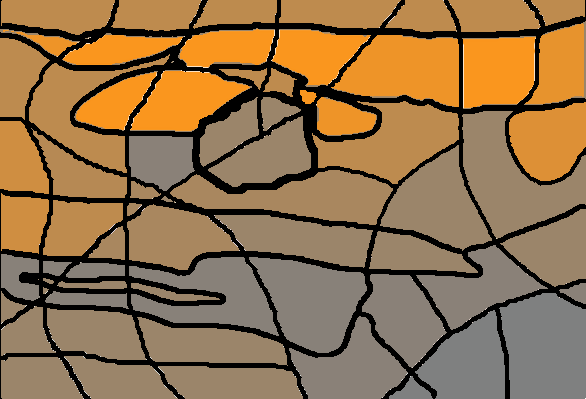
\includegraphics[height=1.9cm]{b.png}}
        \hfill%
        \subfigure[][\tiny $l$ is lungs]{%
          \label{fig:dataTermc}%
        
\includegraphics[height=1.9cm]{c.png}}
        \hspace*{\fill}%
          \subfigure[][\tiny $l$ is lesion]{%
            \label{fig:dataTermd}%
          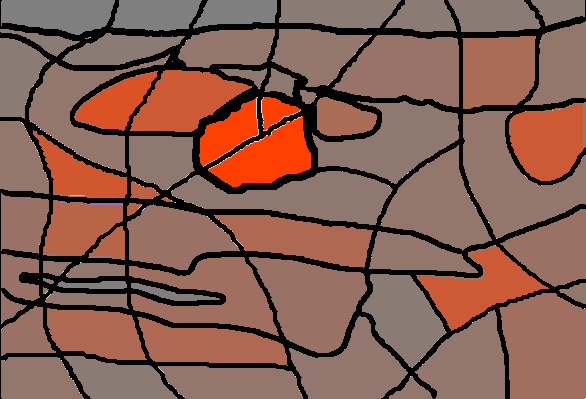
\includegraphics[height=1.9cm]{d.png}}
          \hspace*{\fill}%
            \label{fig:dataTerm}%
    \end{figure}
  \end{block}
	\vspace{-5pt}
  \begin{block}{$V_{s,r}(\omega_s,\omega_r)$ Interpretation}\tiny
  \begin{figure}%
     \centering
     \hspace*{\fill}%
     \subfigure[]{%
       \label{fig:smoothTermb}%
     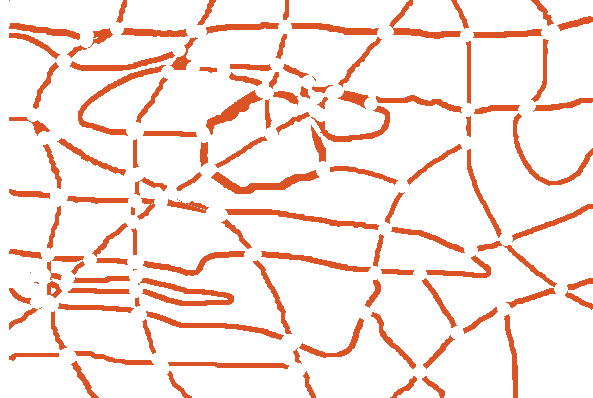
\includegraphics[height=1.9cm]{e.png}}
     \hfill%
     \subfigure[]{%
       \label{fig:smoothTermc}%
     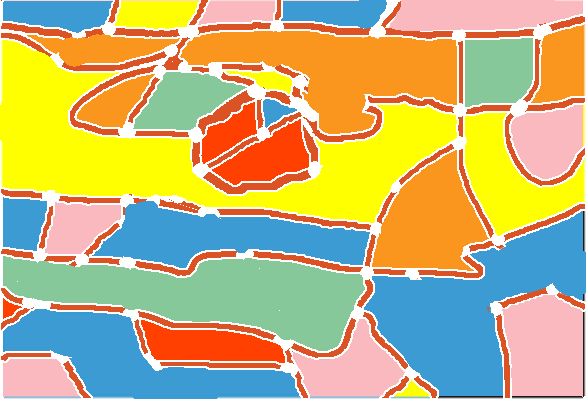
\includegraphics[height=1.9cm]{f.png}}
       \hspace*{\fill}%
     \subfigure[]{%
       \label{fig:smoothTermd}%
     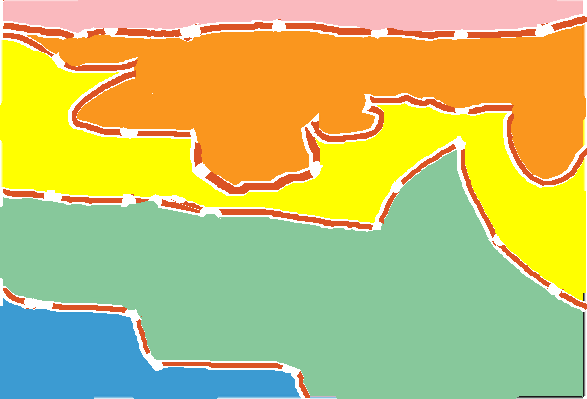
\includegraphics[height=1.9cm]{g.png}}
       \hspace*{\fill}%
    \label{fig:smoothTerm}%
  \end{figure}
\end{block}
	\end{footnotesize}
}

\subsection{System Configuration}
\frame{\frametitle{The Metric Labeling Problem}%\framesubtitle{\insertsubsection}
  \framesubtitle{System Configuration}

\begin{table}[b]
  \caption{Design choices summary}
  \label{tab:method}
  % \begin{tabular}{>{\centering\bfseries}m{1in} l}
  \begin{tabular}{cl} \hline
		$\mathcal{S}$ & {\footnotesize Quick-Shift super-pixels} \\
								&{\footnotesize  Background Echotexture: encoded in Appearance and SIFT-BoW}\\
		$D(\cdot)$ & {\footnotesize Echo Pattern: encoded in Appearance, Atlas and Brightness}\\% \tikz[inner sep=0mm, outer sep=0mm]{\node[inner sep=0mm, outer sep=0mm, anchor=south west] {\includegraphics[height=40pt]{featAll}};} \\
						 & {\footnotesize Acoustic Posterior: encoded in Atlas and Brightness}\\
	$V(\cdot,\cdot)$ & {\footnotesize Homogeneity }\\
		$\arg \min U(\cdot)$ & {\footnotesize Graph-Cuts} \\ \hline
  \end{tabular}
  % % \begin{tabular}{lll}
  % %  $\mathcal{S}$: Quick-Shift super-pixels &\quad &$D(\cdot)$: \\
  % %  $\arg \min:$ Graph-Cuts&&\quad Features \tikz[remember picture]{\coordinate[remember picture] (featCoord) at (0,0);}\\
  % %  $V(\cdot,\cdot)$: homogeneity as Eq.\,\eqref{eq:smoothing}& & \quad Construction { \acs{svm}-\acs{rbf}} \\
  % % \end{tabular}
\end{table}
}
